\documentclass[leqno,DIV=calc,paper=a4,fontsize=11pt]{article}

\usepackage[margin=1in]{geometry}
\setlength{\oddsidemargin}{0mm}					% Adjusting margins to center the colorbox, ...
\setlength{\evensidemargin}{0mm}					% ... you might want to change these
\usepackage[all]{xy}
\usepackage[english]{babel}
\usepackage[protrusion=true,expansion=true]{microtype}	
\usepackage{amsmath,amsfonts,amsthm,amssymb}
\usepackage{graphicx}
\usepackage{mdwtab,booktabs}
\usepackage{pifont}
\usepackage{tikz}
\usetikzlibrary{arrows,chains,matrix,positioning,scopes}
\usepackage{xcolor}
\usepackage{fix-cm}
\usepackage{hyperref}
\hypersetup{colorlinks,linkcolor={blue},citecolor={blue},urlcolor={red}}
% various theorems, numbered by section

\newtheorem{thm}{Theorem}[section]
\newtheorem{lem}[thm]{Lemma}
\newtheorem{prop}[thm]{Proposition}
\newtheorem{cor}[thm]{Corollary}
\newtheorem{conj}[thm]{Conjecture}

\theoremstyle{definition}
\newtheorem{defn}[thm]{Definition}
\newtheorem{defns}[thm]{Definitions}
\newtheorem{con}[thm]{Construction}
\newtheorem{exmp}[thm]{Example}
\newtheorem{notn}[thm]{Notation}
\newtheorem{notns}[thm]{Notations}
\newtheorem{addm}[thm]{Addendum}
\newtheorem{exer}[thm]{Exercise}
\newtheorem{rem}[thm]{Remark}
\theoremstyle{plain}


\theoremstyle{remark}
\newtheorem{rems}[thm]{Remarks}
\newtheorem{warn}[thm]{Warning}
\newtheorem{sch}[thm]{Scholium}
\DeclareMathOperator{\id}{id}
% ------------------------------------------------------------------------------
% Definitions (do not change this)
% ------------------------------------------------------------------------------
\newcommand{\HRule}[1]{\hfill \rule{0.2\linewidth}{#1}} 	% Horizontal rule

\definecolor{grey}{rgb}{0.9,0.9,0.9}

\makeatletter							% Title
\def\printtitle{%						
    {\centering \@title\par}}
\makeatother									

\makeatletter							% Author
\def\printauthor{%					
    {\centering \large \@author}}				
\makeatother							

%%% Headers and footers
\usepackage{fancyhdr}												% Needed to define custom headers/footers
	\pagestyle{fancy}												% Enabling the custom headers/footers
\usepackage{lastpage}	

% Header (empty)
\lhead{}
\chead{}
\rhead{}
% Footer (you may change this to your own needs)
\lfoot{\footnotesize \texttt{www.albohessab.weebly.com} \textbullet }
\cfoot{\thepage}
\rfoot{\footnotesize Miliyon T.}	% "Page 1 of 2"
\renewcommand{\headrulewidth}{0.0pt}
\renewcommand{\footrulewidth}{0.4pt}

% ------------------------------------------------------------------------------
% Metadata (Change this)
% ------------------------------------------------------------------------------
\title{	\fontsize{50}{60}\selectfont
			\vspace*{0.7cm}
            \hfill Algebra Note	\\[0.8cm]
		}

\author{
		\hfill Miliyon T.\\	
		\hfill Addis Ababa University\\	
		\hfill Department of Mathematics\\
        \hfill \texttt{http://www.albohessab.weebly.com} \\
}


\begin{document}
% ------------------------------------------------------------------------------
% Maketitle
% ------------------------------------------------------------------------------
\thispagestyle{empty}				% Remove page numbering on this page

\colorbox{grey}{
	\parbox[t]{1.0\linewidth}{
		\printtitle
		\vspace*{0.5cm}
	}
}

  	\vfill
\printauthor								% Print the author data as defined above
\HRule{1pt}
\clearpage
% ------------------------------------------------------------------------------
% Begin document (Content goes below)
% ------------------------------------------------------------------------------
\tableofcontents
\newpage
\section{Introduction}

\subsection{Sets}\index{Sets}
\begin{defn}[Equality of sets]\index{Sets!Equality of sets}
For any two sets $A$ and $B$; $A=B\Leftrightarrow A\subseteq B$ and $B\subseteq A$.
\end{defn}

\subsection{Functions}
Let $f:A\to B$. Then the diagram of functions

\begin{center}
\begin{tikzpicture}[scale=0.8][!htb]
\node at (1.5,2) [above] {$f$};
\node at (0.25,0.65) {$h$};
\node at (2.75,0.65) {$g$};
\draw [->] (0,2)  node [left] {$A$} -- (3,2) node [right] {$B$};
\node at (1.5,0) [below] {$C$};
\draw [->] (0,1.7) -- (1.3,0);
\draw [<-] (1.7,0) -- (3,1.7);
\end{tikzpicture}
\end{center}
is said to be commutative if $g\circ f=h$. Similarly, the diagram

\begin{center}
\begin{tikzpicture}[scale=0.8][!htb]
\node at (1.5,2) [above] {$f$};
\node at (1.5,-.1) [below] {$k$};
\node at (-0.5,1) {$h$};
\node at (3.5,1) {$g$};
\draw [->] (0,2)  node [left] {$A$} -- (3,2) node [right] {$B$};
\draw [->] (0,0)  node [left] {$C$} -- (3,0) node [right] {$D$};
\draw [<-] (-0.3,0.3) -- (-0.3,1.8);
\draw [<-] (3.3,0.3) -- (3.3,1.8);
\end{tikzpicture}
\end{center}
is said to be commutative if $g\circ f=k\circ h$.\\
If $f:A\to B$
\begin{enumerate}
  \item $S\subset A,\ f(S)=\{f(x):x\in S\}.$
  \item $T\subset B,\ f^{-1}(T)=\{x\in A: f(x)\in T\}.$
  \item $S\subset A\Rightarrow S\subset f^{-1}(f(S))$. If $f$ is $1-1$, then $S=f^{-1}(f(S))$.
  \item $T\subset B \Rightarrow  T\subset f(f^{-1}(T))$. If $f$ is onto, then $T=f(f^{-1}(T))$.
\end{enumerate}
If $A\xrightarrow{f} B\xrightarrow{g} C$, then $g\circ f:A\to C$
\begin{enumerate}
  \item If $f,g$ is $1-1$, so is $g\circ f$.
  \item If $f,g$ is onto, $g\circ f$ is onto.
\end{enumerate}

\begin{defn}[Equivalence relation]\index{Sets!Equivalence relation}
A relation $R$ on a set $A$ is an equivalence relation if it satisfies
\begin{description}
  \item[(i)] Reflexive: $(a,a)\in R,\ \forall a\in A$.
  \item[(ii)] Symmetric: $(a,b)\in R\Rightarrow (b,a)\in R,\ \forall a,b\in A$.
  \item[(iii)] Transitive: $(a,b),(b,c)\in R\Rightarrow (a,c)\in R,\ \forall a,b,c\in A$.
\end{description}
\end{defn}
\begin{defn}
$\bar{a}=\{x\in A:x\thicksim a\}=\{x\in A:(x,a)\in R\}$ is the equivalence class determined by $a$.
$$\bar{a}=\bar{b}\Leftrightarrow a\thicksim b\ i.e. (a,b)\in R.$$
\end{defn}

\begin{prop}
For any $a,b\in A$ either $\bar{a}=\bar{b}$ or $\bar{a}\cap\bar{b}=\emptyset$.
\end{prop}
\begin{defn}
$A/R=$ The set of all equivalence class in $A$.
\end{defn}
\begin{exmp}
Let $m>0$ be an integer. Congruence modulo $m$ is an equivalence relation on $\Bbb Z$ which has precisely $m$ equivalence classes.
\end{exmp}

\begin{defn}[Choice]
Let $A_i:i\in I$ be a non-empty family of sets indexed by $I$. The cartesian product of the sets $A_i$ is the set of all functions
$$f:I\to \bigcup_{i\in I}A_i$$
such that $f(i)\in A_i\ \forall i\in I$. It is denoted by $\prod_{i\in I}A_i$
$$\prod_{i\in I}A_i=\{f:f:I\to \cup A_i\text{ such that }f(i)\in A_i\}.$$
\end{defn}
\begin{defn}[WOA]
Every non empty subset of positive integer has a least element.
\end{defn}
\begin{defn}[PMI]

\end{defn}
\begin{thm}[Division Algorithm]
If $a,b\in \Bbb Z$ and $b\neq 0$, then $\exists!$ integers $q,r$ such that
$$a=qb+r,\qquad 0\leq r<|b|.$$
\end{thm}

\begin{thm}[Bezout's Lemma]

\end{thm}

\newpage
\section{Groups}
\subsection{Basic Definitions}
\begin{defn}[Binary operation]\index{Groups}\index{Groups!Binary operation}
Let $G\neq \emptyset$ a binary operation on $G$ is a function from $G\times G\to G$.
\end{defn}

\begin{defn}[Groupoid]\index{Groups!Groupoid}
A non-empty set $G$ together with a binary operation on $G$.
\end{defn}

\begin{defn}[Semi-Group]\index{Groups!Semi-Group}
A non-empty set $G$ together with a binary operation on $G$ which is associative.
\end{defn}

\begin{defn}[Monoid]\index{Groups!Monoid}
A semi group which contains a two sided identity.
\end{defn}

\begin{defn}[Group]\index{Groups!Group}
A Monoid $G$ such that for every $a\in G$, there exists a two sided inverse.
\end{defn}

\begin{notn}
$|G|=$ order of the group. If $|G|<\infty$, then $G$ is finite otherwise infinite.
\end{notn}

\begin{thm}
If $G$ is a monoid the identity element $e$ is unique
\end{thm}

\begin{proof}
Let $e$ and $e'$ be two identity elements, then
$$e=ee'=e'e=e'$$
\end{proof}

\begin{thm}
If $G$ is a group, then
\begin{description}
  \item[i)] $c\in G$ and $cc=c\Rightarrow c=e.$
  \item[ii)] $\forall a,b,c$
  \begin{align*}
  ab=ac\Rightarrow b=c\tag{Left cancelation}\\
  ba=ca\Rightarrow b=c\tag{Right cancelation}
  \end{align*}
  \item[iii)] For each $a\in G$ the inverse is unique.
  \item[iv)] For each $a\in G$, $(a^{-1})^{-1}=a.$
  \item[v)] For all $a,b\in G$, $(ab)^{-1}=b^{-1}a^{-1}$
  \item[vi)] For all $a,b\in G$, the equation $ax=b$, $ya=b$ have a unique solution $x=a^{-1}b$ and $y=ba^{-1}$.
\end{description}
\end{thm}

\begin{prop}
Let $G$ be a semigroup. Then $G$ is a group iff
\begin{enumerate}
  \item $\exists e\in G$ such that $ea=a,\ \forall a\in G$.
  \item For each $a\in G$, there exists $a^{-1}\in G$ such that $a^{-1}a=e$.
\end{enumerate}
\end{prop}
\begin{proof}

\end{proof}

\begin{prop}
Let $G$ be a semigroup. Then $G$ is a group iff the equations $ax=b$ and $ya=b$ have solutions in $G$.

\end{prop}

\begin{proof}

\end{proof}

\begin{exmp}
$(\Bbb Z,+),(\Bbb Q,+),(\Bbb R,+)$ are groups.\\
$(\Bbb Z,\cdot),(\Bbb Q,\cdot),(\Bbb R,\cdot)$ are monoids.
\end{exmp}

\begin{exmp}
Consider a square with vertices consecutively numbered $1,2,3,4$ and centered at the origin of the $x,y$ plane.
Let $D_4^{*}=\{R,R^2,R^3,I,T_x,T_y,T_{1,3},T_{2,4}\}$
where

\begin{minipage}{0.5\textwidth}
\scriptsize
\begin{align*}
R &\text{ is a counter clockwise rotation about } 90^{\circ}\\
R^2& \text{ is a counter clockwise rotation about } 180^{\circ}\\
R^3& \text{ is a counter clockwise rotation about } 270^{\circ}\\
I &\text{ is a counter clockwise rotation about } 360^{\circ}\\
T_x& \text{ is a reflection about } x-\text{axis}\\
T_y &\text{ is a reflection about } y-\text{axis}\\
T_{1,3}& \text{ is a reflection about the line through } 1\& 3\\
T_{2,4}& \text{ is a reflection about the line through } 2\& 4
\end{align*}
\end{minipage}
\begin{minipage}{0.5\textwidth}
\includegraphics[width=.9\textwidth]{D4.png}
\end{minipage}

\begin{align*}I=\left(
    \begin{matrix}
      1 & 2 & 3 &4\\
      1 & 2 & 3 &4
    \end{matrix}
    \right),\ R=\left(
    \begin{matrix}
      1 & 2 & 3 &4\\
      4 & 1 & 2 &3
    \end{matrix}
    \right),\ R^2=\left(
    \begin{matrix}
      1 & 2 & 3 &4\\
      3 & 4 & 1 &2
    \end{matrix}
    \right),\ R^3=\left(
    \begin{matrix}
      1 & 2 & 3 &4\\
      2 & 3 & 4 &1
    \end{matrix}
    \right),\\
    T_{x}=\left(
    \begin{matrix}
      1 & 2 & 3 &4\\
      4 & 3 & 2 &1
    \end{matrix}
    \right),\ T_{y}=\left(
    \begin{matrix}
      1 & 2 & 3 &4\\
      2 & 1 & 4 &3
    \end{matrix}
    \right),\ T_{1,3}=\left(
    \begin{matrix}
      1 & 2 & 3 &4\\
      1 & 4 & 3 &2
    \end{matrix}
    \right),\ T_{2,4}=\left(
    \begin{matrix}
      1 & 2 & 3 &4\\
      3 & 2 & 1 &4
    \end{matrix}
    \right)
\end{align*}
For $v,u\in D_{4}^{*}$, $uv=u\circ v$ transformation $v$ followed by $u$. Claim: $D_{4}^{*}$ is a non-abelian group of order 8.\\
The Cayley Table for $D_4^{*}$ is

\begin{table}[!htb]
\centering
\begin{tabular}{ | l |c|c|c|c|c|c|c| r | }
    \hline
    $\circ $  & $I$       & $R$       & $R^2$     & $R^3$     & $T_x$     & $T_y$     & $T_{1,3}$ & $T_{2,4}$ \\ \hline
    $I$       & $I$       & $R$       & $R^2$     & $R^3$     & $T_x$     & $T_y$     & $T_{1,3}$ & $T_{2,4}$ \\ \hline
    $R$       & $R$       & $R^2$     & $R^3$     & $I$       & $T_{2,4}$ & $T_{1,3}$ & $T_x$     & $T_y$     \\ \hline
    $R^2$     & $R^2$     & $R^3$     & $I$       & $R$       & $T_y$     & $T_x$     & $T_{2,4}$ & $T_{1,3}$ \\ \hline
    $R^3$     & $R^3$     & $I$       & $R$       & $R^2$     & $T_{1,3}$ & $T_{2,4}$ & $T_y$     & $T_x$     \\ \hline
    $T_x$     & $T_x$     & $T_{1,3}$ & $T_y$     & $T_{2,4}$ & $I$       & $R^2$     & $R$       & $R^3$     \\ \hline
    $T_y$     & $T_y$     & $T_{2,4}$ & $T_y$     & $T_{1,3}$ & $R^2$     & $I$       & $R^3$     & $R$       \\ \hline
    $T_{1,3}$ & $T_{1,3}$ & $T_y$     & $T_{2,4}$ & $T_x$     & $R^3$     & $R$       & $I$       & $R^2$     \\ \hline
    $T_{2,4}$ & $T_{2,4}$ & $T_x$     & $T_{1,3}$ & $T_y$     & $R$       & $R^3$     & $R^2$     & $I$       \\ \hline
  \end{tabular}
  \caption{$(D_4^{*},\circ)$ [$uv$: $u$ from row and $v$ from column.]}
\end{table}
\end{exmp}

\subsection{Homomorphisms}
\begin{defn}
Let $G$ and $H$ be semigroups. A function $f:G\to H$ is a homomorphism if $$f(ab)=f(a)f(b),\qquad \forall a,b\in G.$$
\end{defn}
If $f$ is \textbf{injective}, then $f$ is a \textbf{monomorphism}. If $f$ is \textbf{surjective}, then $f$ is an \textbf{epimorphism}. If $f$ is \textbf{bijective}, then $f$ is an \textbf{isomorphism}.
\begin{defn}
$G$ and $H$ are said to be isomorphic if there is an isomorphism between them.
\end{defn}

\begin{notn}
If $G$ and $H$ are isomorphic we write $G\cong H$.
\end{notn}
\begin{defn}
A homomorphism $f:G\to G$ is called an endomorphism.
\end{defn}
\begin{defn}
An isomorphism $f:G\to G$ is called an automorphism.
\end{defn}
\begin{lem}
If $G$ and $H$ are groups with identities $e_G$ and $e_H$ respectively, then\\
i) $f(e_G)=e_H$.\\
ii) $f(a^{-1})=[f(a)]^{-1}$
\end{lem}

\begin{proof}
Exercise
\end{proof}

 \begin{exmp}
 Let $G$ be an abelian group. Define $f:G\to G$ by $f(x)=x^2$. Show that $f$ is a homomorphism.
 \end{exmp}
 \begin{exmp}
 Define $f:G\to G$ by $f(x)=x^{-1}$. Show that $f$ is an automorphism.
 \end{exmp}
 \begin{defn}
 Let $f:G\to H$ be a homomorphism of groups, then
 $\ker f=\{x\in G:\ f(x)=e\}$\\
 $A\subset G,\ f(A)=\{f(x):x\in A\}$\\
 $B\subset H,\ f^{-1}(B)=\{x\in G:f(x\in B)\}$
 \end{defn}

 \begin{thm}
 If $f:G\to H$ is a homomorphism of groups, then\\
 \begin{enumerate}
   \item $f$ is a monomorphism iff $\ker f=\{e\}$.
   \item $f$ is an isomorphism iff $\exists$  a homomorphism $f^{-1}:H\to G$ such that $f\circ f^{-1}=I_H$ and $f^{-1}f=I_G$.
 \end{enumerate}
 \end{thm}
\begin{proof}
(1) Exercise\\
(2) ($\Rightarrow$) Suppose $f$ is an isomorphism i.e. $f$ is $1-1$, onto, monomorphism. Since $f$ is bijective, there exist $f^{-1}$ which is also bijective.\\
Claim: $f^{-1}$ is homomorphism.
\end{proof}

\subsection{Subgroups}
\begin{defn}
Let $G$ be a group and $\emptyset\neq H\subset G$ that is closed under the binary operation of $G$, then $H$ is said to be a subgroup of $G$ if $H$ by itself is a group.
\end{defn}
\begin{notn}
If $H$ is a subgroup of $G$, we write $H\leq G$.
\end{notn}
\begin{exmp}[Trivial subgroups]
Let $G$ be a group, then $\{e\}$ and $G$ are subgroups of $G$.
\end{exmp}
\begin{exmp}
Consider $(\Bbb Z, +)$, then for $k\in \Bbb Z$, $(k\Bbb Z,+)\leq (\Bbb Z,+)$.
\end{exmp}
\begin{exmp}
Consider $(\Bbb Z_6,\oplus_6)$

\end{exmp}

\begin{prop}
If $p$ is prime, then $\Bbb Z_p$  has no proper subgroups.
\end{prop}

\begin{thm}
Let $f:G\to H$ be a homomorphism of groups, then
\begin{enumerate}
  \item $\ker f\leq G$,
  \item $A\leq G\Rightarrow f(A)\leq H$, (In particular; $im f\leq H$)
  \item $B\leq H\Rightarrow f^{-}(B)\leq G.$
\end{enumerate}
\end{thm}
\begin{proof}
Exercise
\end{proof}

\begin{exmp}
Let $G$ be a group $Aut (G)=\{f:G\to G, f \text{ is an isomorphism}\}$. Show $(Aut(G),\circ)$ is a group.
\end{exmp}

\begin{thm}
Let $\emptyset\neq H\subset G$, $H\leq G$ iff $ab^{-1}\in H,\forall a,b\in H$.
\end{thm}

\begin{cor}
Let $G$ be a group and $\{H_i:i\in \Delta\}$ be a non-emptyset family of subgroups of $G$. Then $\bigcap_{i\in \Delta}\leq G$.
\end{cor}

\begin{defn}
Let $G$ be a group and $X\subset G$. Let $\{H_i:i\in \Delta\}$ be a non-emptyset family of subgroups of $G$ containing $X$(i.e. $X\subset H_i,\forall i\in \Delta$). Then $\bigcap_{i\in \Delta}H_i$ is called the subgroup of $G$ generated by the set $X$ and denoted by $\langle X\rangle$.
\end{defn}
\begin{notn}
If $X=\{a_1,a_2,\ldots,a_n\}$, then $\langle X\rangle=\langle a_1,a_2,\ldots,a_n\rangle$.
\end{notn}

\begin{defn}
If $G=\langle a_1,a_2,\ldots,a_n\rangle$, then we say that $G$ is finitely generated.
\end{defn}
\begin{rem}
$\langle \emptyset\rangle =\{e\}$.
\end{rem}

\begin{thm}
Let $G$ be a group and $\emptyset\neq X\subset G$. Then $\langle X\rangle$ consists of all finite products $a_1^{n_1}a_2^{n_2}\cdots a_t^{n_t}$ where $a_i\in X$ and $n_i\in \Bbb Z$.\\
In particular, for all $a\in G$, $\langle a\rangle=\{a^n:n\in \Bbb Z\}$.
\end{thm}

\subsection{Cyclic groups}

\begin{defn}
A group $G$ is said to be cyclic if $G=\langle a\rangle$ for some $a\in G$.
\end{defn}
\begin{prop}
The only subgroups of $(\Bbb Z,+)$ are of the form $(k\Bbb Z,+)$ for $k\in \Bbb Z$.
\end{prop}

\begin{exmp}
$\Bbb Z=\langle 1\rangle =\langle -1\rangle\Rightarrow \Bbb Z$ is cyclic.
\end{exmp}
\begin{exmp}
The group $\{1,-1,i,-i\}$ under multiplication is a cyclic group.
\end{exmp}

\begin{thm}
Every infinite cyclic group is isomorphic to the additive group $\Bbb Z$ and every finite cyclic group of order $m$ is isomorphic to the additive group $\Bbb Z_m$.
\end{thm}

\begin{proof}
Let $G$ be a cyclic group. Then $G=\langle a\rangle$. Define $\alpha:\Bbb Z\to G$ by $\alpha(k)=a^{k}$.
Claim :- $\alpha$ is an epimorphism.\\
i) Homomorphism: $\alpha(k_1+k_2)=a^{k_1+k_2}=a^{k_1}\cdot a^{k_2}=\alpha(k_1)\alpha(k_2)$
ii) Onto: Let $x\in \langle a\rangle$. Then $x=a^k$ for some $k\in \Bbb Z\Rightarrow \alpha(k)=x$.\\
Hence $\alpha$ is an epimorphism.\\
Consider $\ker \alpha$\\

\end{proof}

\subsection{Permutations}
\begin{defn}
Let $I_n=\{1,2,\ldots,n\}$. $S_n=\{\sigma| \sigma:I_n\to I_n \text{ bijective}\}$. The elements of $S_n$ are called \textbf{permutations}.
\end{defn}

\begin{defn}
Let $i_1,i_2,\ldots,i_r\ (r\leq n)$ be distinct elements of $I_n$. Then $(i_1i_2\cdots i_r)$ denotes a permutation that maps $i_1\to i_2,i_2\to i_3,\cdots,i_{r-1}\to i_r$ and fixes every other element. $(i_1i_2\cdots i_r)$ is called a cycle of length $r$. A cycle of length two is called \textbf{transposition}.
\end{defn}

\begin{defn}
The permutations $\sigma_1,\sigma_2,\ldots,\sigma_r$ of $S_n$ are said to be \textbf{disjoint} for each $1\leq i\leq r$ and every $k\in I_n$ if
$$\sigma_i(k)\neq k\Rightarrow \sigma_j(k)=k,\text{ for every } j\neq i.$$
\end{defn}
\begin{thm}
If $\tau$ and $\sigma$ are disjoint, then $\tau\sigma=\sigma\tau$.
\end{thm}

\begin{proof}
First assume $\sigma(i)\ne i$. Then $\tau(i)=i$ by definition because $\sigma$ and $\tau$ are disjoint, and therefore $\sigma(\tau(i))=\sigma(i)$. On the other hand, because permutations are injective, $\sigma(i)\ne i$ means that $\sigma(\sigma(i))\ne\sigma(i)$, so $\tau(\sigma(i))=\sigma(i)$, again because $\sigma$ and $\tau$ are disjoint. Since $\sigma\tau(i)$ and $\tau\sigma(i)$ both equal $\sigma(i)$, they are equal.

Next assume $\sigma(i)=i$. Then it may be that $\tau(i)\ne i$, in which case proceed as in the previous case with $\tau$ and $\sigma$ interchanged.

Finally if $\sigma(i)=i$ and $\tau(i)=i$, then obviously $\sigma\tau(i)=i=\tau\sigma(i)$.

Since there's always one of these cases that holds, and $\sigma\tau(i)=\tau\sigma(i)$ in each of them, it holds always.
\end{proof}
\begin{thm}
Every non-identity
\end{thm}

\begin{cor}
Every permutation in $S_n$
\end{cor}

\begin{defn}
A permutation $\tau\in S_n$ is said to be \textbf{even}(resp. \textbf{odd}) if $\tau$ can be written as a product of \textbf{even}(resp. \textbf{odd}) number of transpositions.
\[\text{sgn}(\tau)=
\begin{cases}
1 \qquad \text{if } \tau \text{ is even.}\\
-1\qquad \text{if } \tau \text{ is odd.}
\end{cases}
\]
\end{defn}
\begin{thm}
A permutation in $S_n(n\geq2)$ can not be both even and odd.
\end{thm}

\begin{thm}
For each $n\geq2$, let $A_n$ be the set of all even permutations of $S_n$. Then
\begin{description}
  \item[i)] $A_n\lhd S_n$
  \item[ii)] $[S_n:A_n]=2$
  \item[iii)] $|A_n|=|S_n|/2=n!/2$
\end{description}
\end{thm}
\begin{proof}
Consider the group $(\{1,-1\},\cdot)$. Define the map $f:S_n\to \{-1,1\}$ by $f(\sigma)=\text{sgn}(\sigma)$.

\end{proof}
\subsection{Isomorphism Theorems}

\begin{thm}[First Isomorphism Theorem]
If $f:G\to H$ is a group homomorphism, then
$$\ker f\lhd G\qquad\text{and}\qquad G/\ker f \cong im\ f$$
i.e. if $\ker f = K$ and $\phi: G/K \to im\ f \leq H$ is given by $\phi : aK \mapsto f (a)$, then $\phi$ is an isomorphism.
\end{thm}
\begin{rem}
The following diagram describes the proof of the first isomorphism theorem, where $\pi : G \to G/K$ is the natural map $\pi : a \mapsto aK$.

\begin{center}
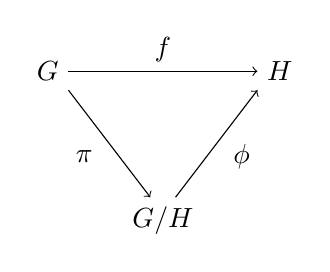
\begin{tikzpicture}[scale=0.8][!htb]
\node at (1.5,2) [above] {$f$};
\node at (0.25,0.65) {$\pi$};
\node at (2.75,0.65) {$\phi$};
\draw [->] (0,2)  node [left] {$G$} -- (3,2) node [right] {$H$};
\node at (1.5,0) [below] {$G/H$};
\draw [->] (0,1.7) -- (1.3,0);
\draw [->] (1.7,0) -- (3,1.7);
\end{tikzpicture}
\end{center}
\end{rem}
\begin{proof}

\end{proof}

\begin{thm}[Second Isomorphism Theorem]
If $N$ and $K$ are subgroups of a group $G$ with $N\lhd G$, then $NK$ is a subgroup, $N \cap K \lhd K$ , and
$$ K/(N \cap K)\cong NK/N.$$
\end{thm}
\begin{proof}

\end{proof}

\begin{thm}[Third Isomorphism Theorem]
If $H$ and $K$ are normal subgroups of a group $G$ with $K \leq H$, then $H/K \lhd G/K$ and
$$(G/K )/(H/K ) \cong G/H.$$
\end{thm}
\begin{proof}

\end{proof}
\subsection{Sylow Theorems}

\begin{thm}[Cauchy] If $G$ is a finite group whose order is divisible by a prime $p$, then $G$ contains an element of order $p$.
\end{thm}

\begin{defn}[$p$-group] A group in which every element has order a power $(\geq 0)$ of some fixed prime $p$ is called a $p$-group. If $H$ is a subgroup of a group $G$ and $H$ is a $p$-group, $H$ is said to be a $p$-subgroup of $G$. In particular $\langle e\rangle$ is a $p$-subgroup of $G$ for every prime $p$ since $|\langle e\rangle| = 1 = p^0$.
\end{defn}

\begin{defn}[Sylow $p$-subgroup] A subgroup $P$ of a group $G$ is said to be a sylow $p$-subgroup of $G$ if $P$ is a maximal $p$ subgroup of $G$. i.e. $P\leq H\leq G$ with $H$ a $p$-subgroup of $G$, then $P=H$.
\end{defn}

\begin{cor}
A finite group $G$ is a $p$-group if and only if $|G|$ is a power of $p$.
\end{cor}

\begin{thm}[First Sylow Theorem] Let $G$ be a group of order p$^nm$, with $n > 1$, $p$ prime, and $(p,n) = 1$. Then $G$ contains a subgroup of order $p^i$ for each $1 < i < n$ and every subgroup of $G$ of order $p^i$ $(i < n)$ is normal in some subgroup of order $p^{i+1}$.
\end{thm}

\begin{cor}
Let $G$ be a group of order $p^nm$ with $p$ prime, $n\geq1$ and $(m,p) = 1$. Let $H$ be a $p$-subgroup of $G$.\\
(i) $H$ is a Sylow $p$-subgroup of $G$ if and only if $|H| = p^n$.\\
(ii) Every conjugate of a Sylow $p$-subgroup is a Sylow $p$-subgroup.\\
(iii) If there is only one Sylow $p$-subgroup $P$, then $P$ is normal in $G$.
\end{cor}

\begin{thm}[Second Sylow Theorem] If $H$ is a $p$-subgroup of a finite group $G$, and $P$ is any Sylow $p$-subgroup of $G$, then there exists $x\in G$ such that $H\leq xPx^{-1}$ In particular, any two Sylow $p$-subgroups of $G$ are conjugate.
\end{thm}

\begin{thm}[Third Sylow Theorem] If $G$ is a finite group and $p$ a prime, then the number of Sylow $p$-subgroups of $G$ divides $|G|$ and is of the form $kp + 1$ for some $k\geq 0$.
\end{thm}

\subsection{Classification of Finite Groups}

We shall classify up to isomorphism all groups of order $pq$ ($p$,$q$ primes) and all groups of small order $n\leq 23$.

\[
\begin{tabular}{clc}
\toprule
Order &   Distinct Groups     \\  \midrule
1     &   $\langle e\rangle$    \\
2     &   $\Bbb Z_2$   \\
3     &   $\Bbb Z_3$    \\
4     &   $\Bbb Z_2\bigoplus\Bbb Z_2$, $\Bbb Z_4$   \\
5     &   $\Bbb Z_5$    \\
6     &   $\Bbb Z_6$, $D_3$   \\
7     &   $\Bbb Z_7$    \\
8     &   $\Bbb Z_2\bigoplus\Bbb Z_2\bigoplus\Bbb Z_2$, $\Bbb Z_2\bigoplus\Bbb Z_4$, $\Bbb Z_8$, $Q_8$, $D_4$   \\
9     &   $\Bbb Z_3\bigoplus\Bbb Z_3$, $\Bbb Z_9$    \\
10    &   $\Bbb Z_{10}$, $D_5$   \\
11    &   $\Bbb Z_{11}$    \\
12    &   $\Bbb Z_2\bigoplus\Bbb Z_6$, $\Bbb Z_{12}$, $A_4$, $D_6$, $T$   \\
13    &   $\Bbb Z_{13}$    \\
14    &   $\Bbb Z_{14}$, $D_7$   \\
15    &   $\Bbb Z_{15}$   \\
16    &   $\Bbb Z_{16}$,    \\
17    &   $\Bbb Z_{17}$,   \\
18    &   $\Bbb Z_{18}$,    \\
19    &   $\Bbb Z_{19}$,   \\
20    &   $\Bbb Z_{20}$,   \\
21    &   $\Bbb Z_{21}$,    \\
22    &   $\Bbb Z_{22}$,   \\
23    &   $\Bbb Z_{23}$,    \\ \bottomrule
\end{tabular}
\]
\newpage
\section{Rings}

\subsection{Definition and elementary properties}
\begin{defn}

\end{defn}

\begin{exmp}

\end{exmp}
\begin{defn}

\end{defn}
\begin{notn}

\end{notn}

\end{document}
